% arara: pdflatex: { shell: true, draft: true }
% arara: makeglossaries
% arara: biber
% arara: pdflatex: { shell: true, synctex: true }
% arara: pdflatex: { shell: true, synctex: true }

\documentclass{f4_beamer_metropolis}

\title{Transport Layer Security 1.3}
\subtitle{SITS WS18/19}
\author{Dennis Grabowski, B.Sc}
\date{28.11.2018}

\bibliography{literature.bib}

\begin{document}

% Cannot be moved into the class
\begin{frame}{Table of contents}
    \tableofcontents[hideallsubsections]
  \end{frame}

\section{Introduction}

\subsection{Motivation}

\begin{frame}{TLS 1.2}
\begin{itemize}
  \item TLS 1.2 was released \textbf{10 years ago}
  \item Last change to specification in RFC6176, released in \textbf{\citeyear{RFC6176}}: \newline
  \textit{\citetitle{RFC6176}}

\end{itemize}
\end{frame}

\begin{frame}{What new, relevant technologies were invented?}
  \begin{itemize}
    \item HTTP Public Key Pinning (HPKP) / Certificate Transparency (CT)
    \item Hash Key Derivation Function (HKDF)
    \item Curve25519 sowie 448
    \item Edwards-curve Digital Signature Algorithm (EdDSA)
  \end{itemize}

  \note{
    Disclaimer: Curve22519 is not a new technology.
    It was released in 2005.
    But after discovery that NSA implemented a backdoor into Dual\_EC\_DRBG, interest increased.
    Since 2017 NIST added them to Special Publication 800-186, allowing the use by US Federal Government.
  }
  \end{frame}

\begin{frame}{What new attacks were discovered?}
Too many to list them all
  \begin{itemize}
    \item Renegotiation attacks
    \item Downgrading attacks: FREAK \& Logjam,
    \item Cross-protocol attacks: DROWN,
    \item Chosen-plaintext attacks: BEAST,
    \item Compression based attacks: CRIME \& BREACH,
    \item Padding oracle attacks: POODLE, Serge Vaudenay's attack,
    \item Timing attacks: Lucky Thirteen,
    \item Attacks on specific ciphers: Sweet32, RC4,
    \item Truncation attacks,
    \item Resumption based attacks,
    \item Implementation errors: Heartbleed, BERserk, Cloudflare,
    \item Attacks which are enabled by TLS: Unholy PAC
  \end{itemize}

  \note{
    RC4 Cipher attacks esp. bad in timing as it was recommended as mitigation against BEAST \\
  }
\end{frame}

\newcolumntype{Y}{>{\centering\arraybackslash}X}
\newcolumntype{S}{>{\centering\small}X}

\subsection{Browser and library support}

\begin{frame}{Which browsers support TLS 1.3?}
  \begin{tabularx}{\textwidth}{
      |>{\hsize=0.2\hsize} Y |
      >{\hsize=0.5\hsize} S |
      >{\hsize=0.2\hsize} Y |
      >{\hsize=0.1\hsize} Y |
    }
    \hline
    \textbf{Browser} & \textbf{Platforms} & \textbf{Versions} & \textbf{TLS 1.3}\\ \hline
    \multirow{2}{*}{Google Chrome}
        & \multirow{2}{*}{\parbox{6cm}{Windows (7+), Linux, Android (4.1+), Chrome OS, macOS (10.10+), iOS (9.0+)}}
          & 54 - 69 & \cellcolor{yellow!50}Disabled \\ \cline{3-4}
    & & 70 & \cellcolor{green!50}Yes \\ \hline
    \multirow{2}{*}[-0.75em]{Mozilla Firefox}
        & \multirow{2}{*}[-0.75em]{\parbox{6cm}{Windows (7+), Linux, Android (4.1+), macOS (10.9+), iOS (9.0+)}}
          & 49 - 62, ESR 52.0 - 60.3 & \cellcolor{yellow!50}Disabled \\ \cline{3-4}
    & & 63 & \cellcolor{green!50}Yes \\ \hline
    Internet Explorer & Windows (7+), Windows Server (2008 R2+) & IE 11 & \cellcolor{red!50}No \\ \hline
    \multirow{2}{*}{Microsoft Edge}
        & Windows 10 Mobile, Xbox & Edge 15 & \cellcolor{red!50}No \\ \cline{2-4}
    & Windows 10, Windows Server (2016+) & Edge 18 & \cellcolor{red!50}No \\ \hline
    Apple Safari & iOS 12, macOS 10.14 & 12 & \cellcolor{yellow!50}Disabled \\ \hline
    Opera Browser & Windows (7+), Linux, Android (4.0+), macOS (10.9+) & 56 & \cellcolor{yellow!50}Disabled \\ \hline
    Tor Browser & Windows (7+), Linux, macOS (10.9+) & IE 11 & \cellcolor{green!50}Yes \\ \hline
    \end{tabularx}

    \note{
      Chrome uses BoringSSL (Google's fork of OpenSSL) \\
      Firefox uses Mozilla's Network Security Services (NSS) \\
      Edge uses Microsoft's EdgeHTML on Windows, Apple/KDE's Webkit on iOS, and Chromium's Blink on Android \\
      Opera uses Apple/KDE's Webkit and Chromium's Blink \\
      Apple Safari apparently allows the use of TLS 1.3, but it is disabled and must be activated with \texttt{defaults write /Library/Preferences/com.apple.networkd tcp_connect_enable_tls13 1}\\
      Tor uses Firefox ESR 60.2 under the hood, which currently only implements the draft-22 version, but they are thinking about backporting NSS changes
    }
\end{frame}

\begin{frame}{Which libraries support TLS 1.3?}
  \begin{tabularx}{\textwidth}{
    |>{\hsize=0.4\hsize} Y |
    >{\hsize=0.2\hsize} Y |
    >{\hsize=0.3\hsize} Y |
    >{\hsize=0.1\hsize} Y |
  }
  \hline
  \textbf{Library} & \textbf{Language} & \textbf{Versions} & \textbf{TLS 1.3}\\ \hline
  BoringSSL & C++ & \texttt{master} & \cellcolor{green!50}Yes \\ \hline
  fizz & C++ & v2018.11.12.00 & \cellcolor{green!50}Yes \\ \hline
  GnuTLS & C & 3.6.3 & \cellcolor{green!50}Yes \\ \hline
  Java Secure Socket Extension & Java & JDK11 & \cellcolor{green!50}Yes \\ \hline
  miTLS & F* & - & \cellcolor{green!50}Yes \\ \hline
  NSS & C / Assembler & 3.39 & \cellcolor{green!50}Yes \\ \hline
  OpenSSL & C & 1.1.1 & \cellcolor{green!50}Yes \\ \hline
  rustls & Rust & 0.14.0 & \cellcolor{green!50}Yes \\ \hline
  SChannel (Windows API) & C++ & Windows 10 v1607 & \cellcolor{red!50}No \\ \hline
  Secure Transport & C / Swift & macOS 10.13, iOS 11 & \cellcolor{yellow!50}Yes \\ \hline
  wolfSSL & C & 3.15 & \cellcolor{green!50}Yes \\ \hline
  \end{tabularx}

  \note{
    cryptlib is a library from Peter Gutmann, a Professor in Auckland \\
    JSSE (Java) will need JDK11, but other library like Bouncy Castle is good too. \\
  }
\end{frame}

\section{Changes to the current protocol}

\subsection{1-RTT Handshake instead 2-RTT}

\begin{frame}{TLS v1.2 Handshake}
  \begin{figure}[!h]
    \centering
    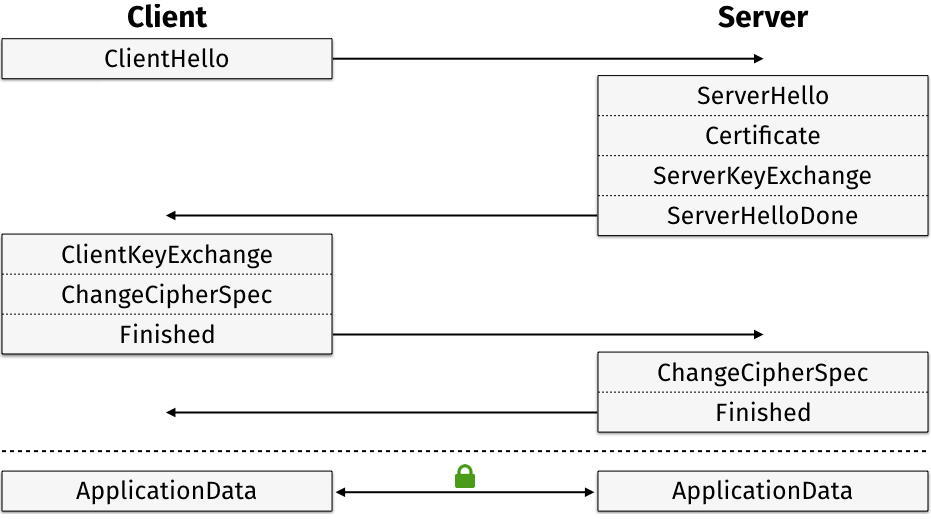
\includegraphics[scale=0.375,keepaspectratio]{./images/tls12-handshake-ecdhe.png}
    %\caption{TLS 1.2 Handshake mit ECDHE}
    \label{fig:tls12-handshake-ecdhe}
  \end{figure}

  \note{
    ECDHE daher, weil static RSA ab TLS 1.3 nicht mehr unterstuetzt ist.
    Bei static RSA wuerde ServerKeyExchange nicht durchgefuehrt werden.
  }
\end{frame}

\begin{frame}[standout]
  TLS v1.2 Handshake - Wiresharkdemo
\end{frame}

\begin{frame}{TLS v1.3 Handshake}
  \begin{figure}[!h]
    \centering
    \vspace*{-0.25cm}
    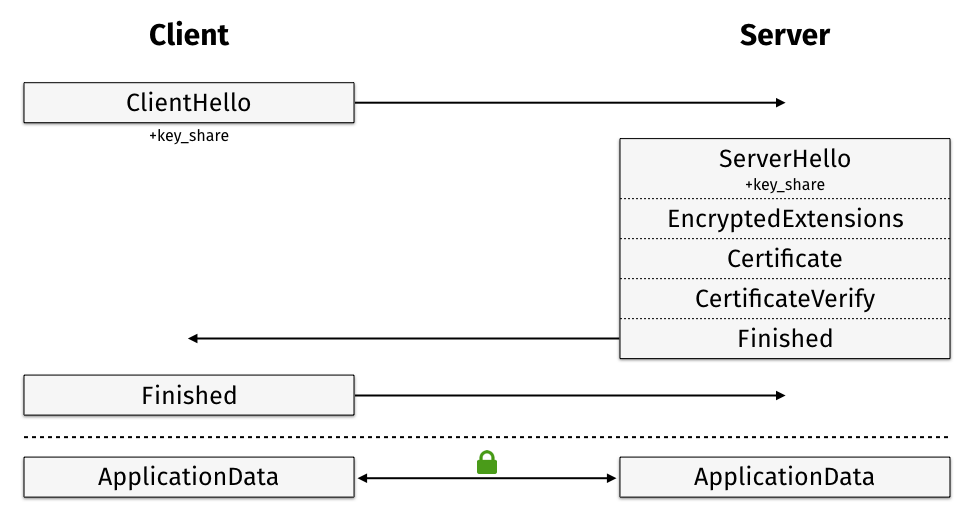
\includegraphics[width=\linewidth]{./images/tls13-handshake-ecdhe.png}
    %\caption{TLS 1.3 Handshake mit ECDHE}
    \label{fig:tls13-handshake-ecdhe}
  \end{figure}
\end{frame}

\begin{frame}[standout]
  TLS v1.3 Handshake - Wiresharkdemo
\end{frame}

\section{New Features coming to TLS 1.3}

\subsection{0-RTT Resumption}

\begin{frame}{0-RTT Handshake}
  \begin{figure}[!h]
    \centering
    \vspace*{-0.25cm}
    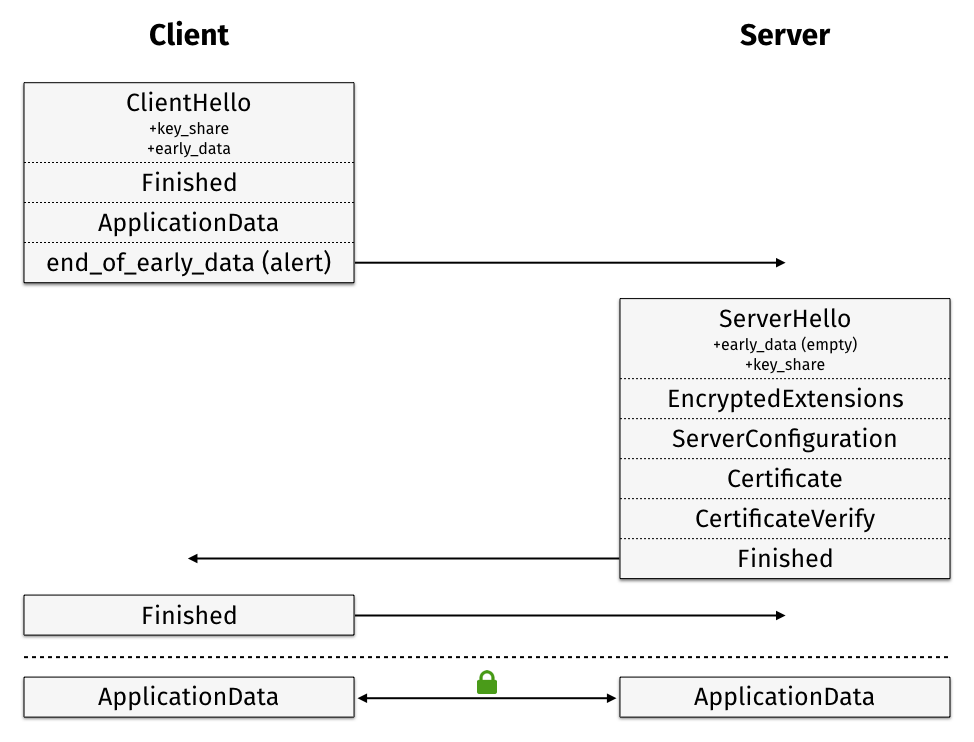
\includegraphics[width=\linewidth]{./images/tls13-handshake-zero-rtt.png}
    %\caption{TLS 1.3 Handshake mit ECDHE}
    \label{fig:tls13-handshake-zero-rtt}
  \end{figure}
\end{frame}

\subsection{Session Resumption}

\begin{frame}{Session Resumption basierend auf einem \enquote{pre-shared key}-Modus}
  \begin{figure}[!h]
    \centering
    \vspace*{-0.25cm}
    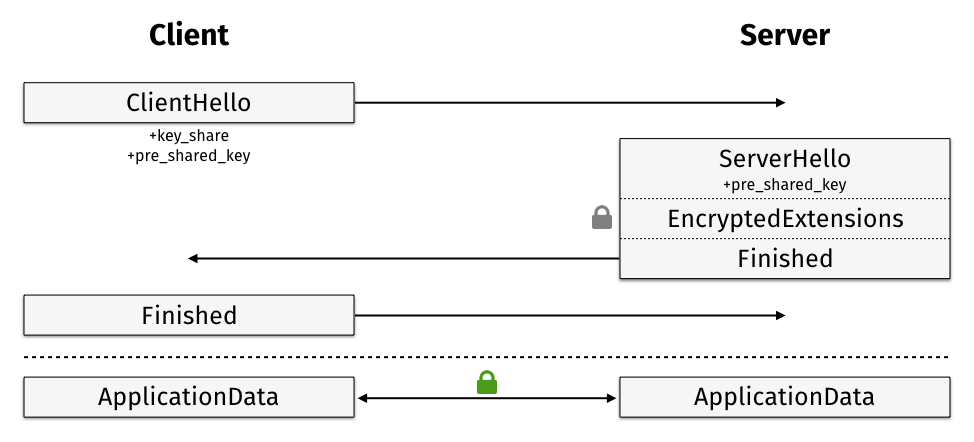
\includegraphics[width=\linewidth]{./images/tls13-handshake-resumption.png}
    %\caption{TLS 1.3 Handshake mit ECDHE}
    \label{fig:tls13-handshake-resumption}
  \end{figure}
\end{frame}

\subsection{Protection from downgrading}

\begin{frame}{What is downgrading?}

\end{frame}

\section{Features, die vereinfacht wurden}

\begin{frame}{}
Festgesetzte DHE Gruppen (wegen LogJam-Angriff)
\end{frame}

\section{Features removed from TLS 1.3}

\subsection{Why do features need to be removed?}

\begin{frame}
  \begin{enumerate}[<+->]
    \item Cipher Suites werden unsicher durch neu-erfundene Attacken
    \item Features stellen sich als unsicher heraus
    \end{enumerate}
\end{frame}

\subsection{Entfernte Cipher Suites und Hashing Funktionen}

\begin{frame}
RC4, SHA1, MD5
\end{frame}

\subsection{Compression}

\begin{frame}
Wegen CRIME Angriff
\end{frame}

\subsection{Renegotiation}

\begin{frame}

\end{frame}

\subsection{Static RSA Handshake}

\begin{frame}
Hierfuer gibts num standardmaessig ECDHE
Static RSA hat keine Forward Perfect Secrecy gegeben
\end{frame}

\subsection{CBC und MAC-then-Encrypt mode}

\begin{frame}
Dafuer gibts nun AEAD
Dadurch werden Attacken Vaudenay, Lucky 13 und POODLE vermieden
\end{frame}

\subsection{RSA PKCS#1v1.5}

\begin{frame}
  RSASSA-PSS als Ersatz
  https://en.wikipedia.org/wiki/Probabilistic_signature_scheme
\end{frame}

\section{Conclusion}

\begin{frame}

\end{frame}

\begin{frame}[standout]
  Questions?
\end{frame}

\section{Literature}

\begin{frame}[allowframebreaks]{Literature}
  \printbibliography
\end{frame}

\appendix

\begin{frame}{Formale Verifikation}

\end{frame}

\end{document}
